\documentclass[tikz]{standalone}

\usepackage[greek,english]{babel}

\usepackage{pgfplots}
\usetikzlibrary{decorations.pathreplacing}

\pagecolor{white}

\begin{document}
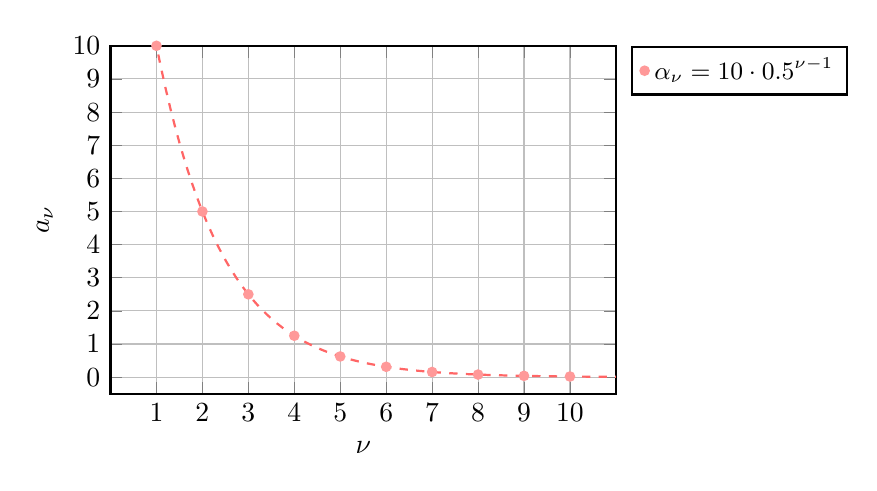
\begin{tikzpicture}
\begin{axis}[
    width=8cm,
    height=6cm,
    domain=-15:15, 
    xmin=0,
    xmax=11,
    ymin=-0.5,
    ymax=10,
    thick,
    ytick={0,1,2,3,4,5,6,7,8,9,10},
    xtick=data,
    legend pos=outer north east,
    mark size=1.5pt,
    xlabel={$\nu$},
    ylabel={$a_\nu$},
    legend cell align={left},
    grid]


\addplot[only marks, red!40!white] coordinates {
(1, 10)
(2, 5)
(3, 2.5)
(4, 1.25)
(5, 0.625)
(6, 0.3125)
(7, 0.15625)
(8, 0.078125)
(9, 0.0390625)
(10, 0.0195312)
};
\addlegendentry{\small $\alpha_\nu = 10 \cdot 0.5^{\nu - 1}$ }

\addplot[red, domain=0.1:11,restrict y to domain=0:1800, samples=100, red!60!white,forget plot,dashed]  {10 * 0.5^(x-1)};


\end{axis}
\end{tikzpicture}
\end{document}
